
%(BEGIN_QUESTION)
% Copyright 2010, Tony R. Kuphaldt, released under the Creative Commons Attribution License (v 1.0)
% This means you may do almost anything with this work of mine, so long as you give me proper credit

Suppose we have an Allen-Bradley MicroLogix 1000 controller connected to three pushbutton switches as shown in this illustration:

$$\includegraphics[width=15.5cm]{i04636x01.eps}$$

Determine the necessary switch actuation statuses (i.e. pressed versus unpressed) to turn the lamp on given the following program running in the PLC:

$$\includegraphics[width=15.5cm]{i04636x02.eps}$$

\underbar{file i04636}
%(END_QUESTION)





%(BEGIN_ANSWER)

Necessary switch statuses:

\begin{itemize}
\item{} Switch A = {\bf pressed}
\item{} Switch B = {\bf pressed}
\item{} Switch C = {\bf released}
\end{itemize}

%(END_ANSWER)





%(BEGIN_NOTES)


%INDEX% PLC, relating I/O status to virtual elements 

%(END_NOTES)


